% Native editable composition from verified, unchanged IDE images.
\begin{figure}[htbp]
  \centering
  \sbox0{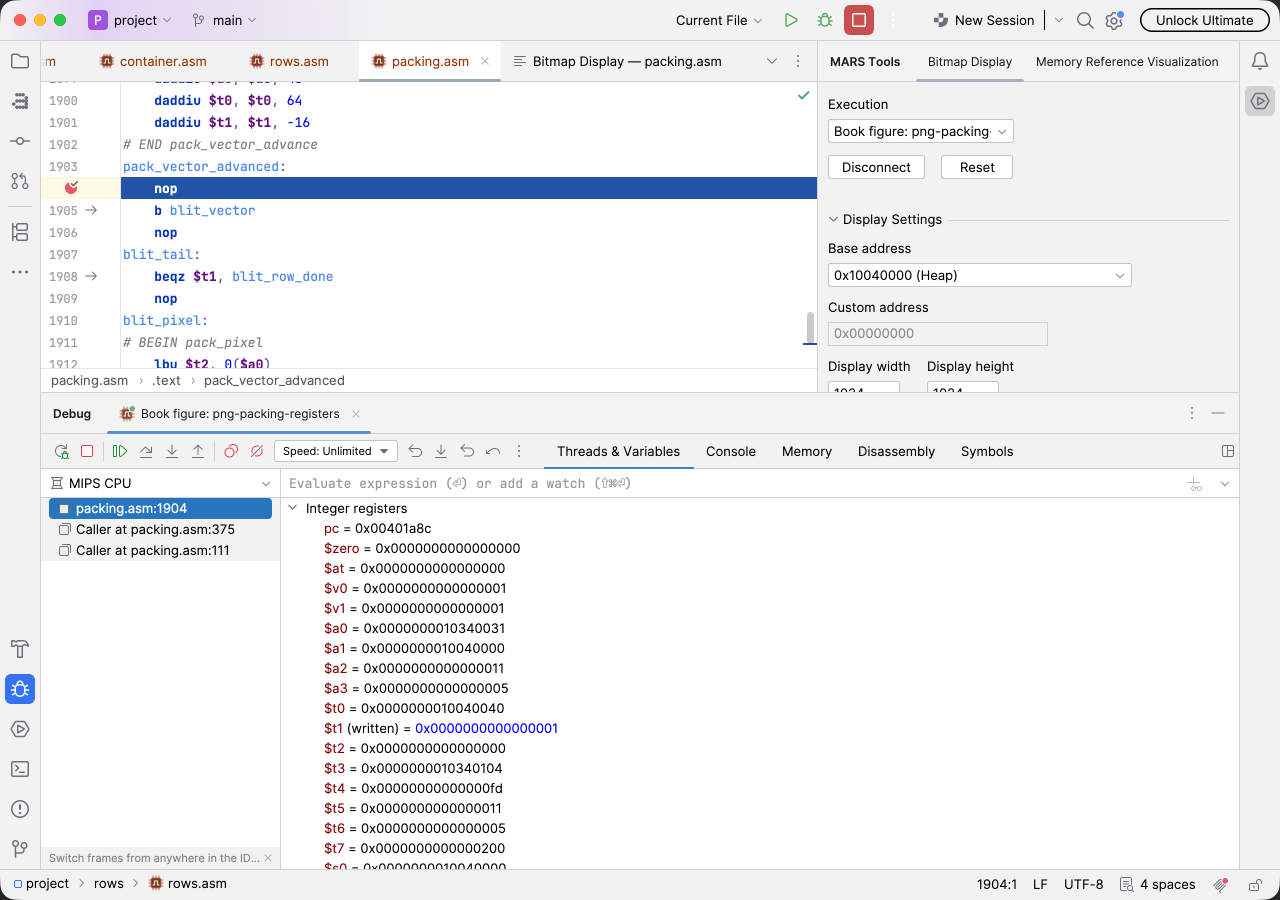
\includegraphics[artifact]{packages/033-png/captures/png-vector-packing/registers.png}}
  \sbox2{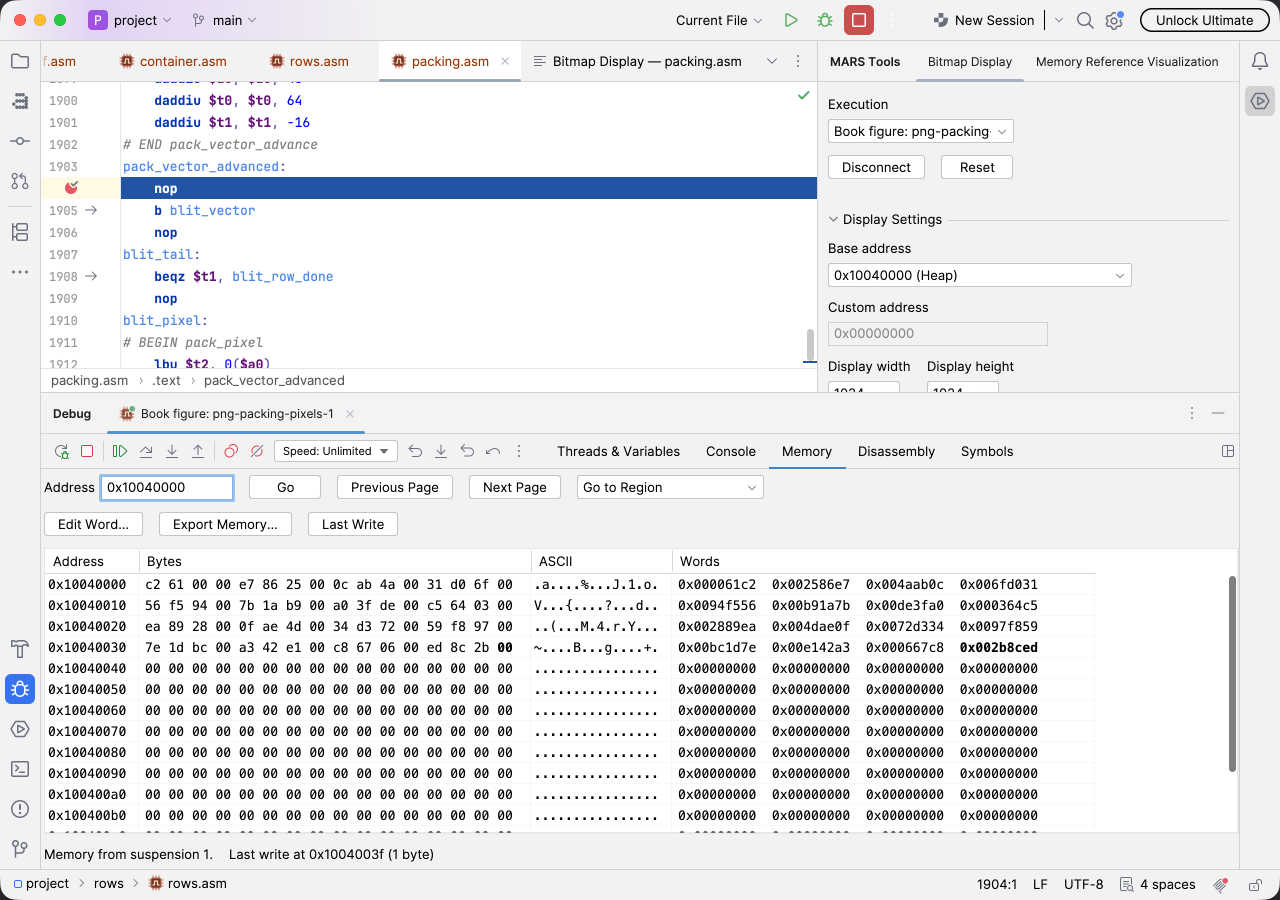
\includegraphics[artifact]{packages/033-png/captures/png-vector-packing/pixels-1.png}}
  \sbox4{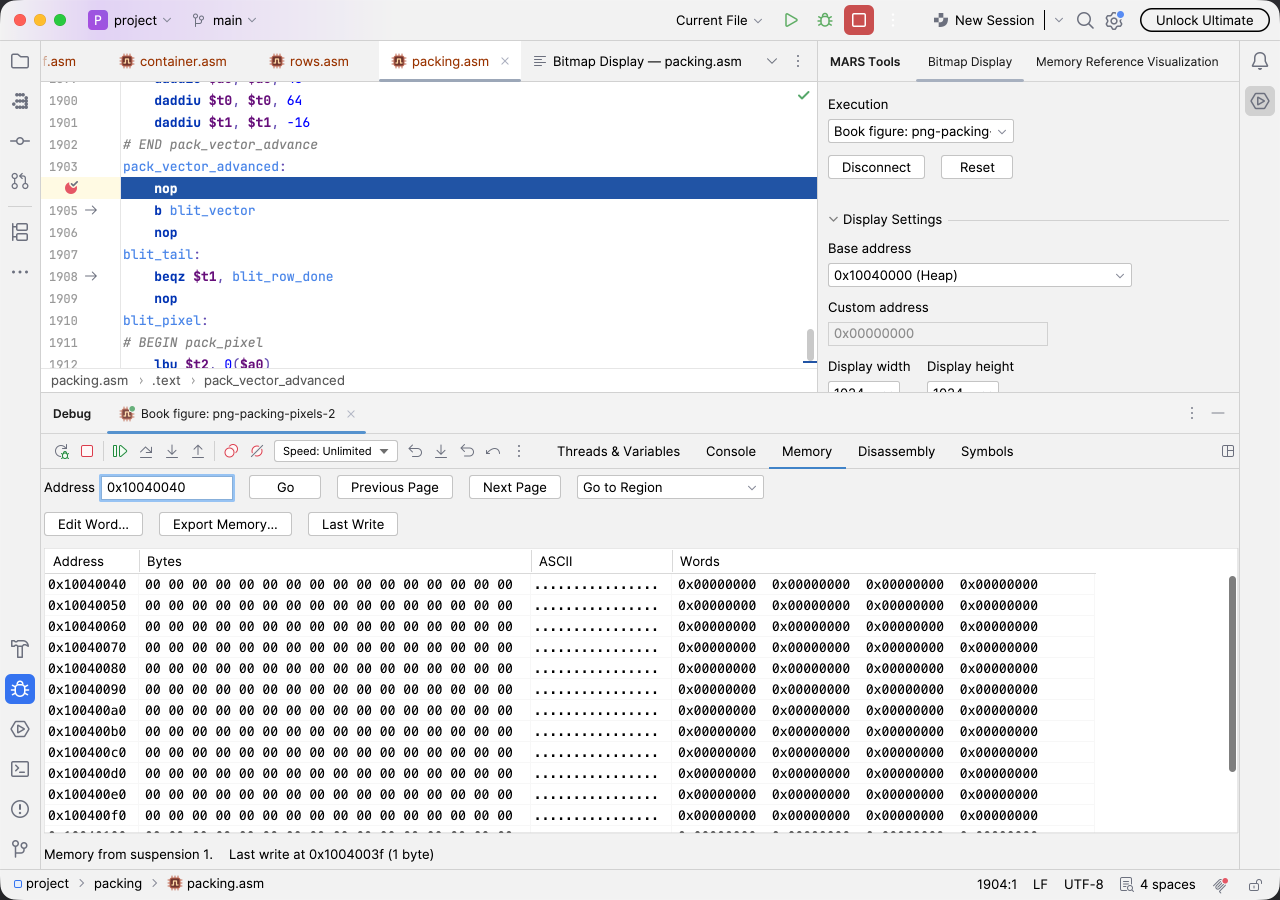
\includegraphics[artifact]{packages/033-png/captures/png-vector-packing/pixels-2.png}}
  \edef\MARSpackingsourceLeft{\the\dimexpr0.036718750\wd0\relax}
  \edef\MARSpackingsourceBottom{\the\dimexpr0.774444444\ht0\relax}
  \edef\MARSpackingsourceRight{\the\dimexpr0.611718750\wd0\relax}
  \edef\MARSpackingsourceTop{\the\dimexpr0.170000000\ht0\relax}
  \edef\MARSpackingpixelsLeft{\the\dimexpr0.520312500\wd2\relax}
  \edef\MARSpackingpixelsBottom{\the\dimexpr0.265555556\ht2\relax}
  \edef\MARSpackingpixelsRight{\the\dimexpr0.139843750\wd2\relax}
  \edef\MARSpackingpixelsTop{\the\dimexpr0.634444444\ht2\relax}
  \edef\MARSpackingtailLeft{\the\dimexpr0.520312500\wd4\relax}
  \edef\MARSpackingtailBottom{\the\dimexpr0.335555556\ht4\relax}
  \edef\MARSpackingtailRight{\the\dimexpr0.139843750\wd4\relax}
  \edef\MARSpackingtailTop{\the\dimexpr0.634444444\ht4\relax}
  \edef\MARSpackingremainingLeft{\the\dimexpr0.246093750\wd0\relax}
  \edef\MARSpackingremainingBottom{\the\dimexpr0.176666667\ht0\relax}
  \edef\MARSpackingremainingRight{\the\dimexpr0.557812500\wd0\relax}
  \edef\MARSpackingremainingTop{\the\dimexpr0.794444444\ht0\relax}
  \begin{tikzpicture}[alt={Four annotated IDE details at pack_vector_advanced before its nop. Sixteen numeric RGB words begin with 0x000061c2 and end with 0x002b8ced. The next destination word remains zero because the seventeenth pixel is pending. Register t1 is one. The source RGB cursor has advanced 48 bytes and the destination cursor 64 bytes.}]
    \node[anchor=north west,inner sep=0,font=\small\bfseries] (source-title) at (6mm,0) {After advancing one complete vector group};
    \node[anchor=north west,inner sep=0] (source) at ([yshift=-1mm]source-title.south west) {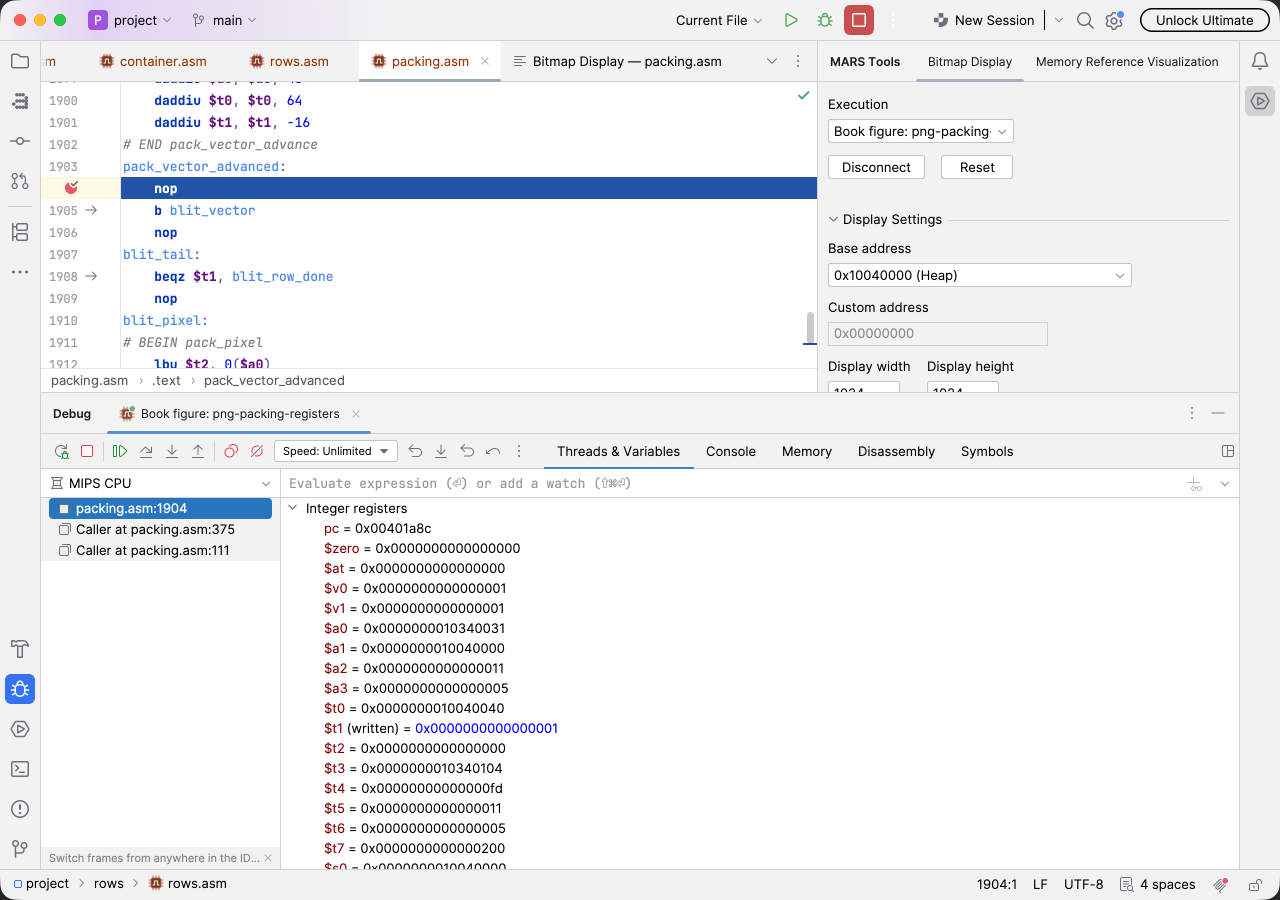
\includegraphics[width=0.7\linewidth,artifact,trim={\MARSpackingsourceLeft{} \MARSpackingsourceBottom{} \MARSpackingsourceRight{} \MARSpackingsourceTop{}},clip]{packages/033-png/captures/png-vector-packing/registers.png}};
    \begin{scope}[shift={(source.south west)},x={($(source.south east)-(source.south west)$)},y={($(source.north west)-(source.south west)$)}]
      \draw[black,line width=0.7pt] (0.168888889,0.080000000) rectangle (0.288888889,0.520000000);
      \node[draw=black,fill=white,circle,inner sep=1.5pt,font=\footnotesize] at ($(0.168888889,0.520000000)+(-3mm,0)$) {1};
    \end{scope}
    \node[anchor=north west,inner sep=0,font=\small\bfseries] (pixels-title) at ([yshift=-2mm]source.south west) {Sixteen numeric RGB words};
    \node[anchor=north west,inner sep=0] (pixels) at ([yshift=-1mm]pixels-title.south west) {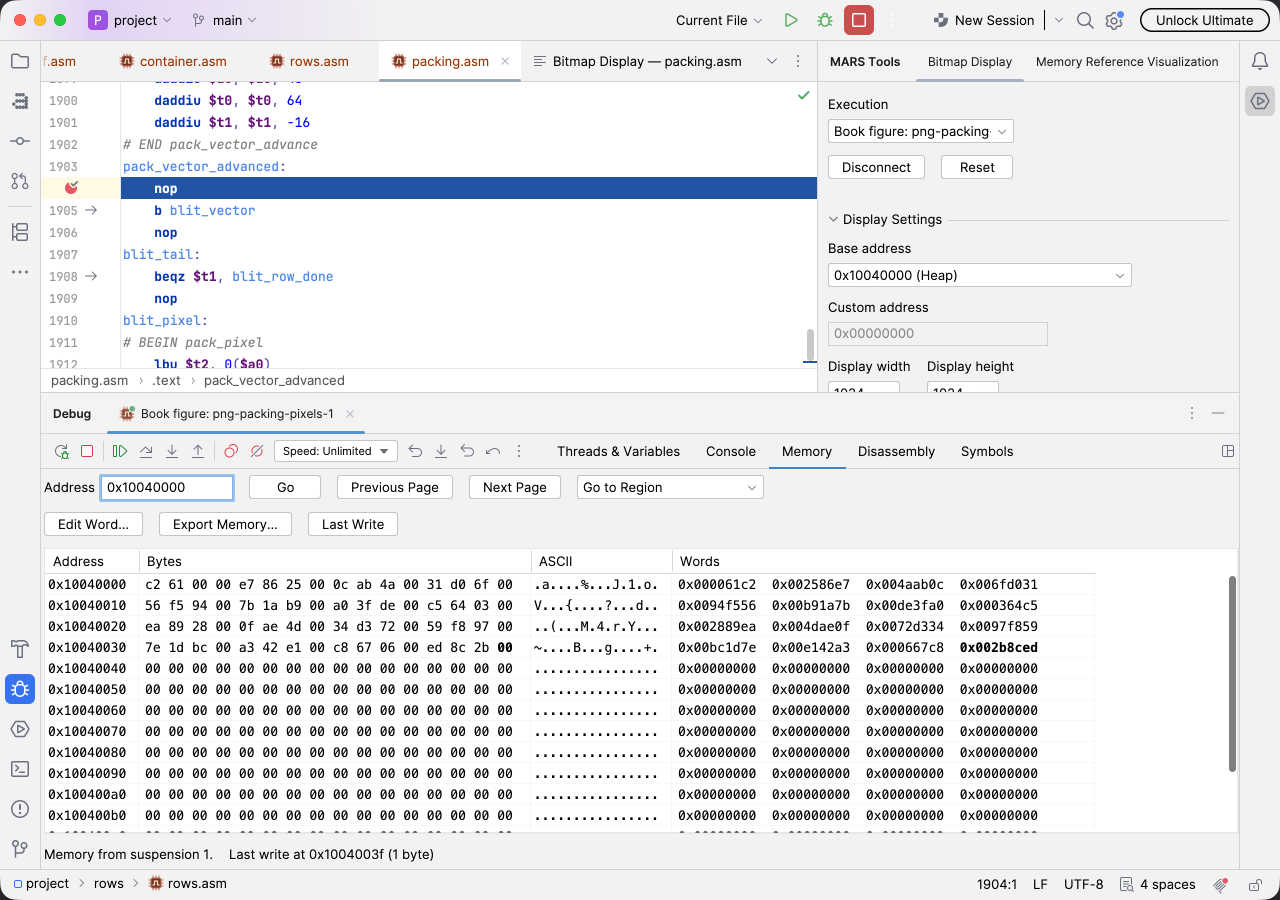
\includegraphics[width=0.84\linewidth,artifact,trim={\MARSpackingpixelsLeft{} \MARSpackingpixelsBottom{} \MARSpackingpixelsRight{} \MARSpackingpixelsTop{}},clip]{packages/033-png/captures/png-vector-packing/pixels-1.png}};
    \begin{scope}[shift={(pixels.south west)},x={($(pixels.south east)-(pixels.south west)$)},y={($(pixels.north west)-(pixels.south west)$)}]
      \draw[black,line width=0.7pt] (0.013793103,0.033333333) rectangle (0.986206897,0.966666667);
      \node[draw=black,fill=white,circle,inner sep=1.5pt,font=\footnotesize] at ($(0.013793103,0.966666667)+(-3mm,0)$) {2};
    \end{scope}
    \node[anchor=north west,inner sep=0,font=\small\bfseries] (tail-title) at ([yshift=-2mm]pixels.south west) {Pending scalar destination word};
    \node[anchor=north west,inner sep=0] (tail) at ([yshift=-1mm]tail-title.south west) {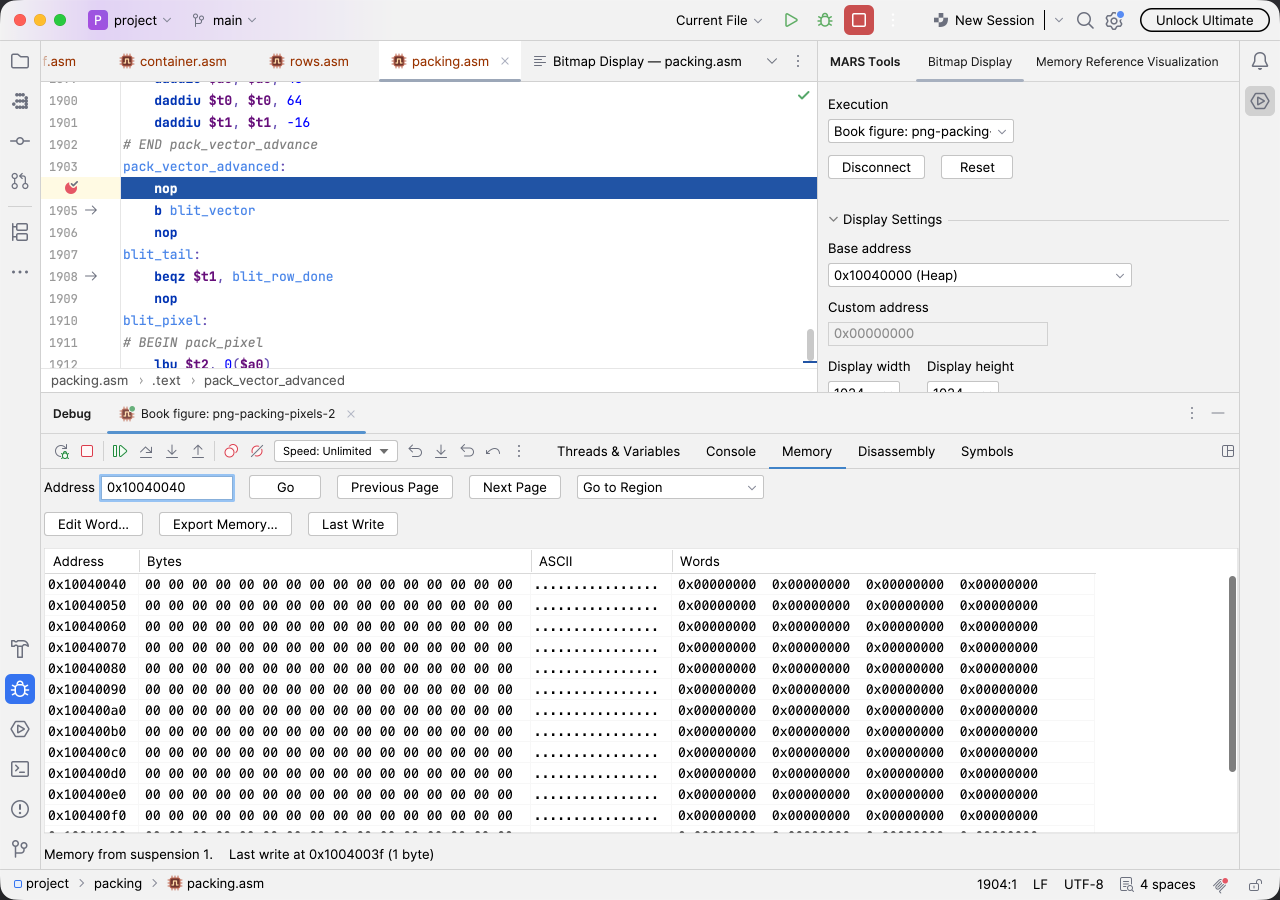
\includegraphics[width=0.84\linewidth,artifact,trim={\MARSpackingtailLeft{} \MARSpackingtailBottom{} \MARSpackingtailRight{} \MARSpackingtailTop{}},clip]{packages/033-png/captures/png-vector-packing/pixels-2.png}};
    \begin{scope}[shift={(tail.south west)},x={($(tail.south east)-(tail.south west)$)},y={($(tail.north west)-(tail.south west)$)}]
      \draw[black,line width=0.7pt] (0.013793103,0.111111111) rectangle (0.986206897,0.888888889);
      \node[draw=black,fill=white,circle,inner sep=1.5pt,font=\footnotesize] at ($(0.013793103,0.888888889)+(-3mm,0)$) {3};
    \end{scope}
    \node[anchor=north west,inner sep=0,font=\small\bfseries] (remaining-title) at ([yshift=-2mm]tail.south west) {One pixel remains in this row};
    \node[anchor=north west,inner sep=0] (remaining) at ([yshift=-1mm]remaining-title.south west) {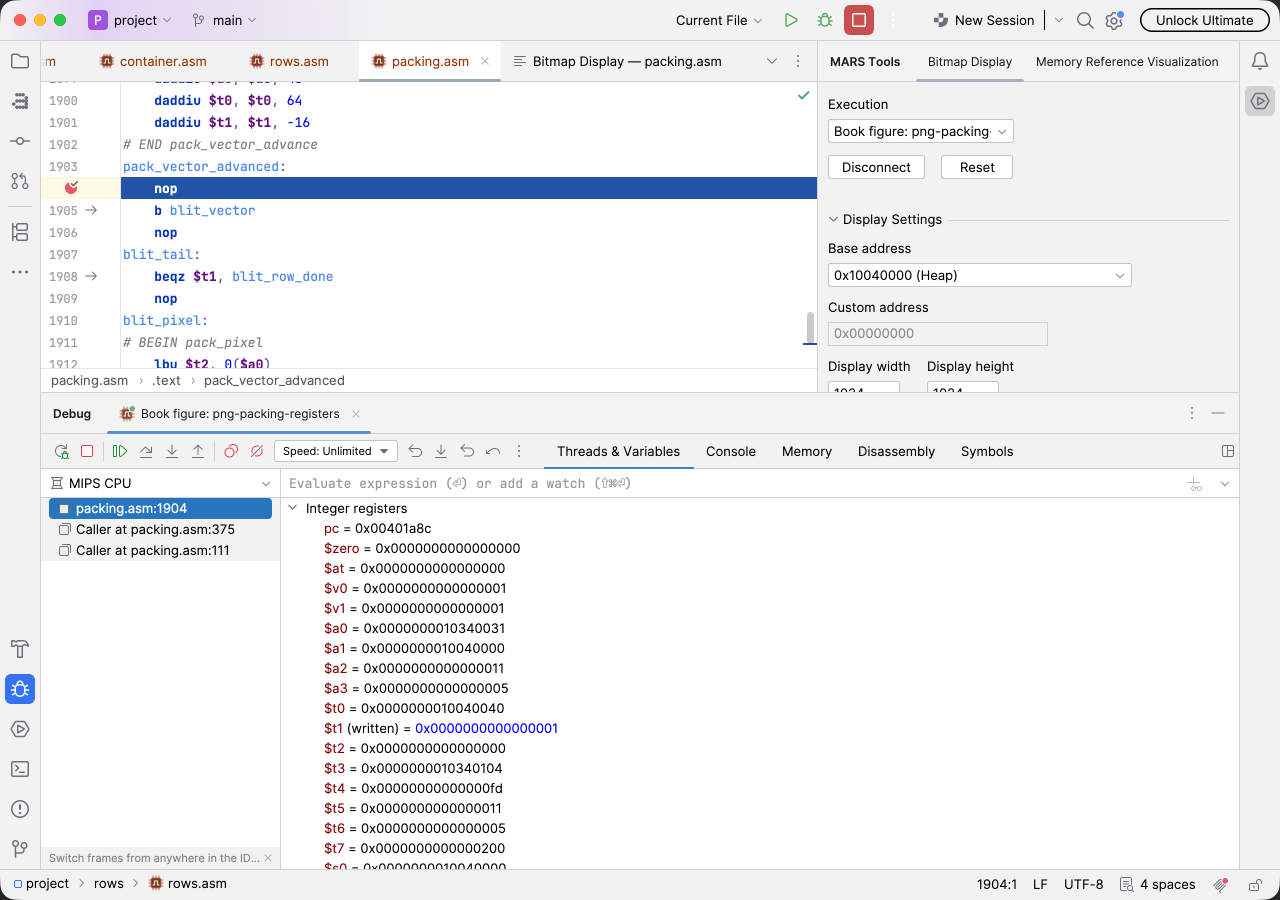
\includegraphics[width=0.5\linewidth,artifact,trim={\MARSpackingremainingLeft{} \MARSpackingremainingBottom{} \MARSpackingremainingRight{} \MARSpackingremainingTop{}},clip]{packages/033-png/captures/png-vector-packing/registers.png}};
    \begin{scope}[shift={(remaining.south west)},x={($(remaining.south east)-(remaining.south west)$)},y={($(remaining.north west)-(remaining.south west)$)}]
      \draw[black,line width=0.7pt] (0.023904382,0.115384615) rectangle (0.976095618,0.884615385);
      \node[draw=black,fill=white,circle,inner sep=1.5pt,font=\footnotesize] at ($(0.023904382,0.884615385)+(-3mm,0)$) {4};
    \end{scope}
  \end{tikzpicture}
  \par\smallskip
  \begin{minipage}{\linewidth}
    \small
    \begin{enumerate}
      \item The RGB cursor has advanced by 48 bytes and the destination cursor by 64. The next group test will select the scalar remainder.
      \item The four rows contain sixteen numeric words, starting with \texttt{0x000061c2}. A native-word store gives the correct numeric color in the configured little-endian target.
      \item The word at framebuffer offset 64 is still zero. It belongs to the seventeenth pixel, whose three source bytes have not yet been consumed.
      \item \texttt{\$t1}=1. This is the illustrated loop remainder, not the completed function return count.
    \end{enumerate}
  \end{minipage}
  \caption{Sixteen vector-packed pixels and one pending scalar pixel in the first row. Three Debug launches share the same source and checkpoint.}
  \label{fig:png-vector-packing}
\end{figure}
